\documentclass[prb,preprint]{revtex4-1} 
% The line above defines the type of LaTeX document.
% Note that AJP uses the same style as Phys. Rev. B (prb).

\usepackage{amsmath}  % needed for \tfrac, \bmatrix, etc.
\usepackage{amsfonts} % needed for bold Greek, Fraktur, and blackboard bold
\usepackage{graphicx} % needed for figures
\usepackage{tabularx}
\usepackage{color}
\DeclareMathOperator{\sinc}{sinc}
\begin{document}

\title{Confirmation of the Wave Nature of Light through the Double-Slit Experiment}
% In a long title you can use \\ to force a line break at a certain location.

\author{Yumeng Melody Cao}
\email{mcao@smith.edu} % optional
% If there were a second author at the same address, we would put another 
% \author{} statement here.  Don't combine multiple authors in a single
% \author statement.
\affiliation{Department of Physics, Smith College, Northampton, MA 01063}
% Please provide a full mailing address here.

\author{He Claudia Yun}
\email{hyun@smith.edu}
\affiliation{Department of Physics, Smith College, Northampton, MA 01063}

% See the REVTeX documentation for more examples of author and affiliation lists.

\date{\today}

%____________abstract____________________________________________

\begin{abstract}
%The motivation of this experiment originates from the interference of light waves caused by 
%originated from that, this experiment we use the TWS apparatus with a laser of wavelength 670nm to re-perform Young's Double-Slit Experiment. 

% shown in Fig.\ref{image}
When a coherent laser beam passes through two narrow slits, these two light beams of a constant phase difference will diffract from each slit and spread out passing through each other. This leads to constructive and destructive interference that can be detected on a screen at some distance from the slits. This phenomenon shows the wave nature of light. 
%This experiment, also known as the Young$^\prime$s double-slit experiment, 
Originally done by Young back in 1800, the double-slit experiment was reproduced in this lab with the use of the TWS apparatus with a laser of 670nm in wavelength. The monochromatic light beam was sent from one end of a u-channel through a double-slit to create an interference pattern. The photodiode at the other end measures the light intensity and by moving a slit across the detector, variations in light intensity can be used to infer the interference pattern. 
%The results and the plots in the experiment successfully demonstrated the wave nature of light. 
The observed interference pattern is fitted using Fraunhofer model, which describes far-field diffraction. The amplitude of the double-slit pattern was observed to be the modulated by the single slit diffraction pattern. Reduced $\chi^2$ of the double-slit fit curve is 0.827 and that of the single-slit fit curve is 1.57, both indicating that the data are consistent with the model within our estimate of uncertainty.

\end{abstract}

\begin{figure}[b]
\centering
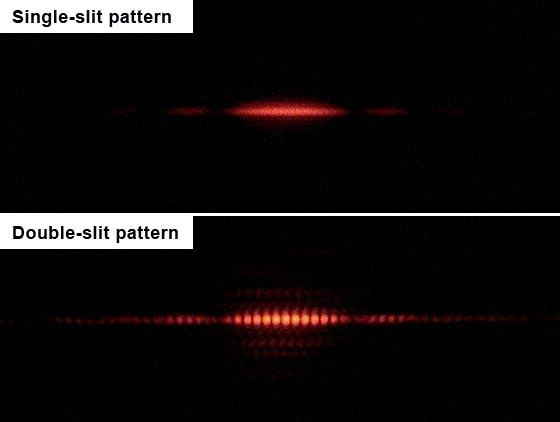
\includegraphics[width=3in]{image1.jpg}
\caption{Single and double-slit interference patterns \cite{wik}.}
%
\includegraphics[width=1in]{white.png}
\label{image}
\end{figure}

\maketitle 

%____________Introduction____________________________________________
\section{Introduction}
The double-slit experiment --- also known as the Young$^\prime$s experiment --- explores the wave-like nature of light. It is important in this experiment that the two sources of light are coherent and have a constant phase difference. Back in 1801, Thomas Young had difficulty with using common light sources, such as candles and lanterns, to be served as coherent sources of light. Thus instead, Young performed the experiment by filtering sunlight through a pinhole in a window shutter split by a piece of card and projecting it horizontally across the room. Light waves from either side of the card coming through the pinhole can be thus considered coherent sources and the interference pattern was then projected onto a screen. (See Fig. \ref{interference})

\begin{figure}[h]
\centering
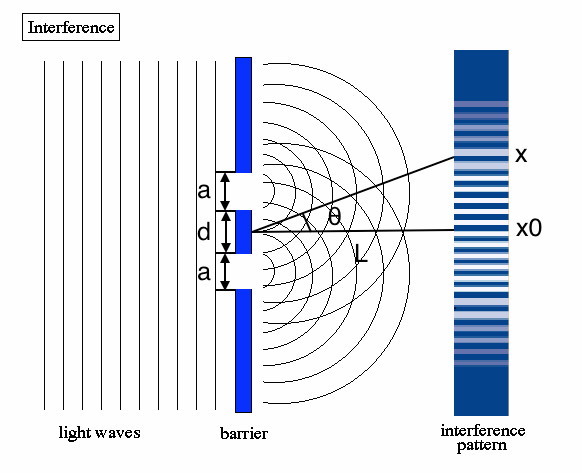
\includegraphics[width=5in]{interference.png}
\caption{Calculate angle from position \cite{interference}. L being the distance between the slits and the photo diode($\approx50cm$); a being the slit width; d being the slit separation; x0 being the location reading on the detector slit micrometer at the central maximum; x being the location reading on the detector slit micrometer at different values to obtain the intensity at that distance from the central maximum; $\theta$ being the angle between the central maximum and value of x. How x is calculated is included in the discussion section. (Eq. \ref{theta}); }
\label{interference}
\end{figure}

First looking at the double slit experiment, to create the curve of best fit, the Fraunhofer equation is applied to the double-slit intensity: 

\begin{equation}
I=I_0 \sinc^2{\left(\frac{\pi a}{\lambda}\sin{\theta}\right)}  \cos^2{\left(\frac{\pi d}{\lambda} \sin \theta\right)}
\label{eq1}
\end{equation}
\begin{equation*}
\sinc(\alpha) \equiv \frac{\sin(\alpha)}{\alpha}
\end{equation*}

The Fraunhofer conditions can be applied once again to create  the curve of best fit for the single-slit experiment: 
\begin{equation}
I=I_0 \sinc^2 \left(\frac{\pi a}{\lambda} \sin\theta \right)
\label{eq2}
\end{equation}

%____________Experiment____________________________________________
\section{Experiment}

A TWS (TWo-Slit) apparatus (Fig. \ref{dia}) is used to perform this experiment. A monochromatics laser is fixed at one end of a U-channel, sending a laser beam with a wavelength of 670 nm through a double slit and the interference pattern is detected by a photodiode at the other end of the light-tight U-channel. Apart from the double-slit, a source-slit, a slit-blocker and a detector-slit are also installed in the U-channel. The source-slit is a single slit with a width narrower than the width of the laser beam, and is used to limit the intensity of the laser beam to decrease the possibility of saturating the detector. The slit-blocker is downstream to the double-slit, and is a wide single slit that can be moved using a micrometer outside the U-channel. The slit-blocker is wide enough to let both ribbons of light pass when it is centered, but it can also be moved to block one or both ribbons. The detector-slit is right in front of the photodiode. It is a narrow single slit, letting a narrow band of the interference pattern pass and detected by the photodiode. By moving the detector-slit through a micrometer outside the U-channel, the intensity of the interference pattern can be measured as a function of the position of the detector-slit x. The shutter at the photodiode end is kept closed to protect the PMT (PhotoMultiplier Tube) behind, which we didn?t use in this experiment. \\


All parts are carefully aligned following the TeachSpin Instruction Manuals for two-slit interference. The laser beam is adjusted to aim directly down the center of the U-channel all the way to the detector, and the slits are adjusted to maximize the intensity of the interference pattern. The key positions of the slit-blocker where it blocks both ribbons of light, blocks one and lets both pass, are recorded. The photodiode is connected to a multimeter which is ultimately connected to the computer. LabView is used to collect data first for the double-slit experiment and for the single-slit experiment. \\

\begin{figure}[h!]
\centering
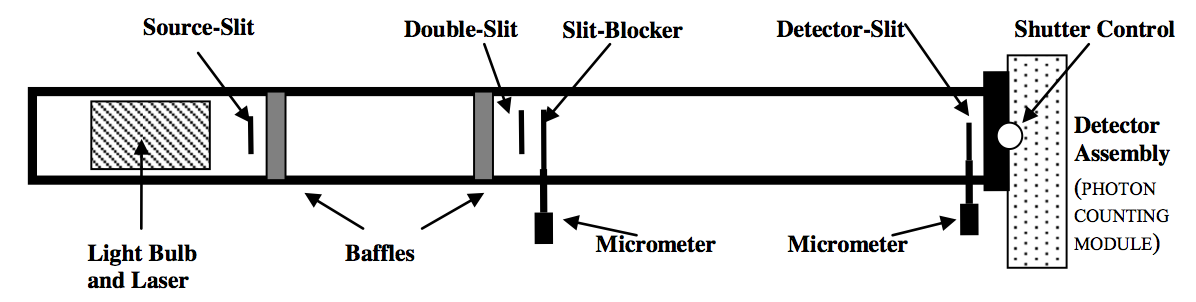
\includegraphics[width=7in]{dia}
\caption{Schematic of TWS apparatus - not to scale \cite{dia}.}
\label{dia}
\end{figure}

After the preparation work, the double-slit experiment is first performed. A double-slit with slit width approximately 0.1 mm and slit separation 0.406 mm is chosen. The slit-blocker is set at the position, where light from both slits are allowed to pass. The photodiode outputs a voltage that is proportional to the intensity of the interference pattern. By changing the position of the detector-slit, intensity of the interference pattern is recorded by LabView as a function of location. Then the experiment is repeated for single-slit when the slit-blocker is moved to block light from one of the two slits. \\
%____________Results____________________________________________
\section{Results}

\begin{figure}[h]
\centering
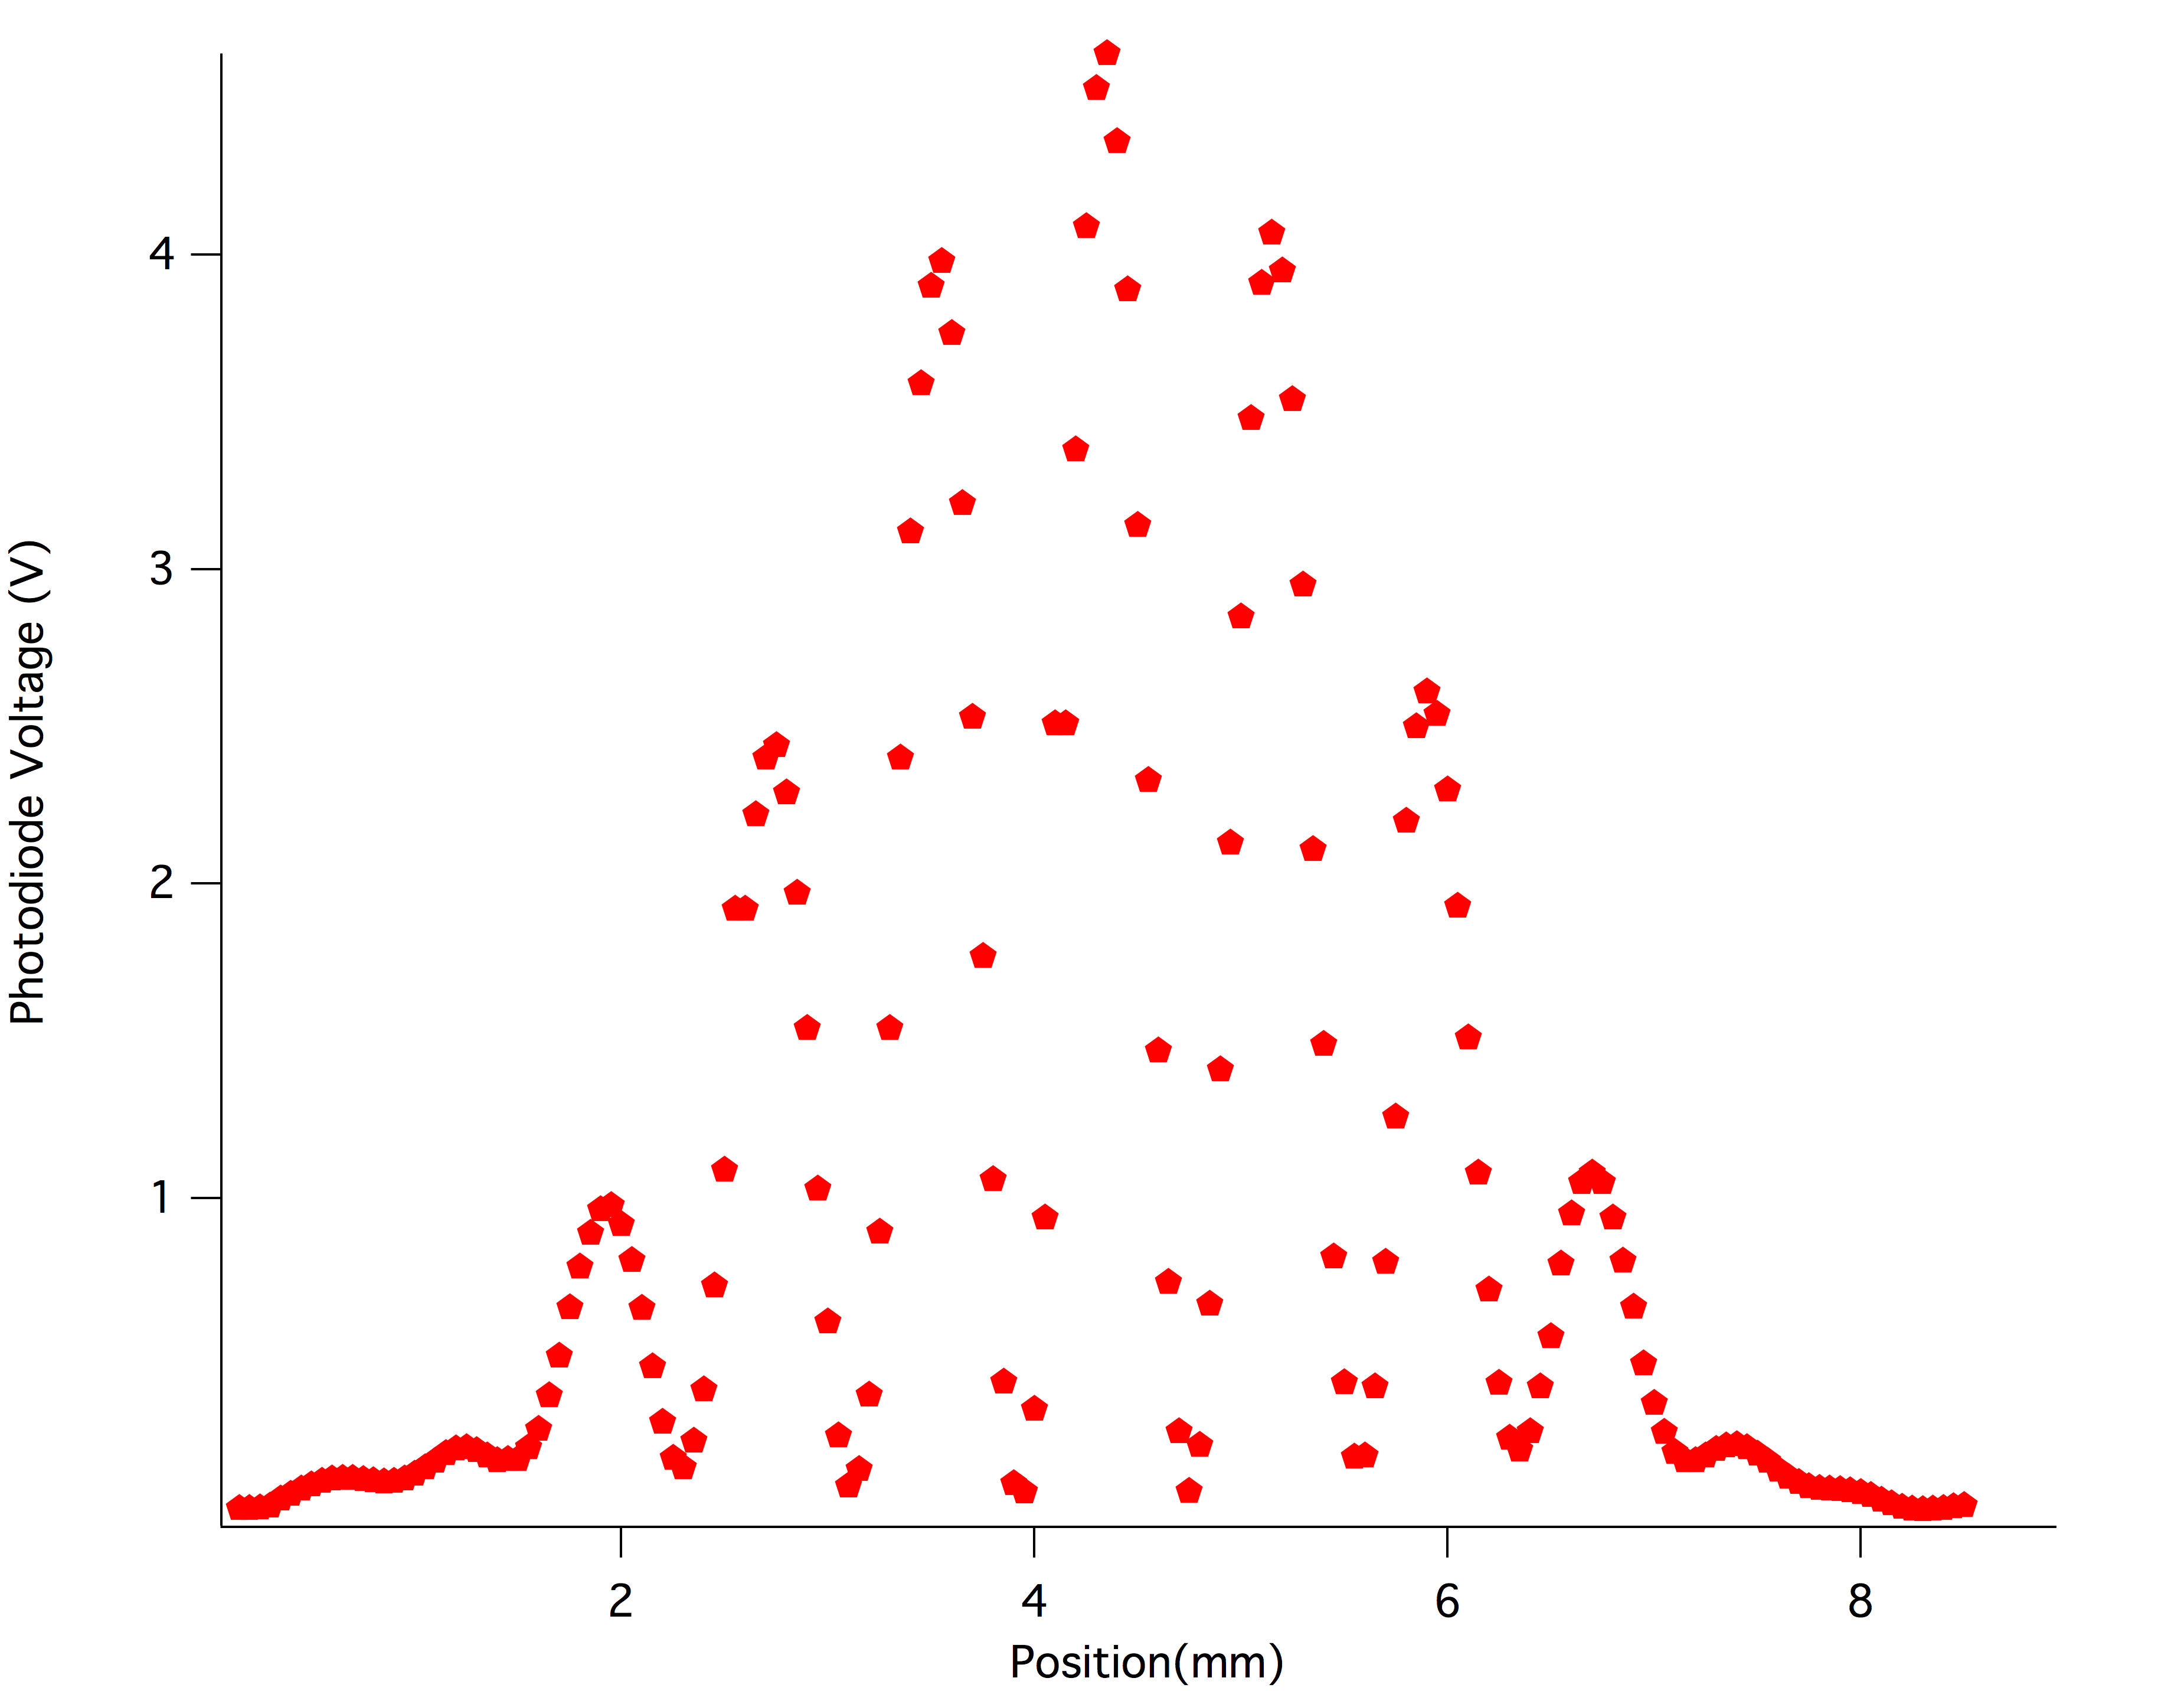
\includegraphics[width=3.2in]{doubleres.png}
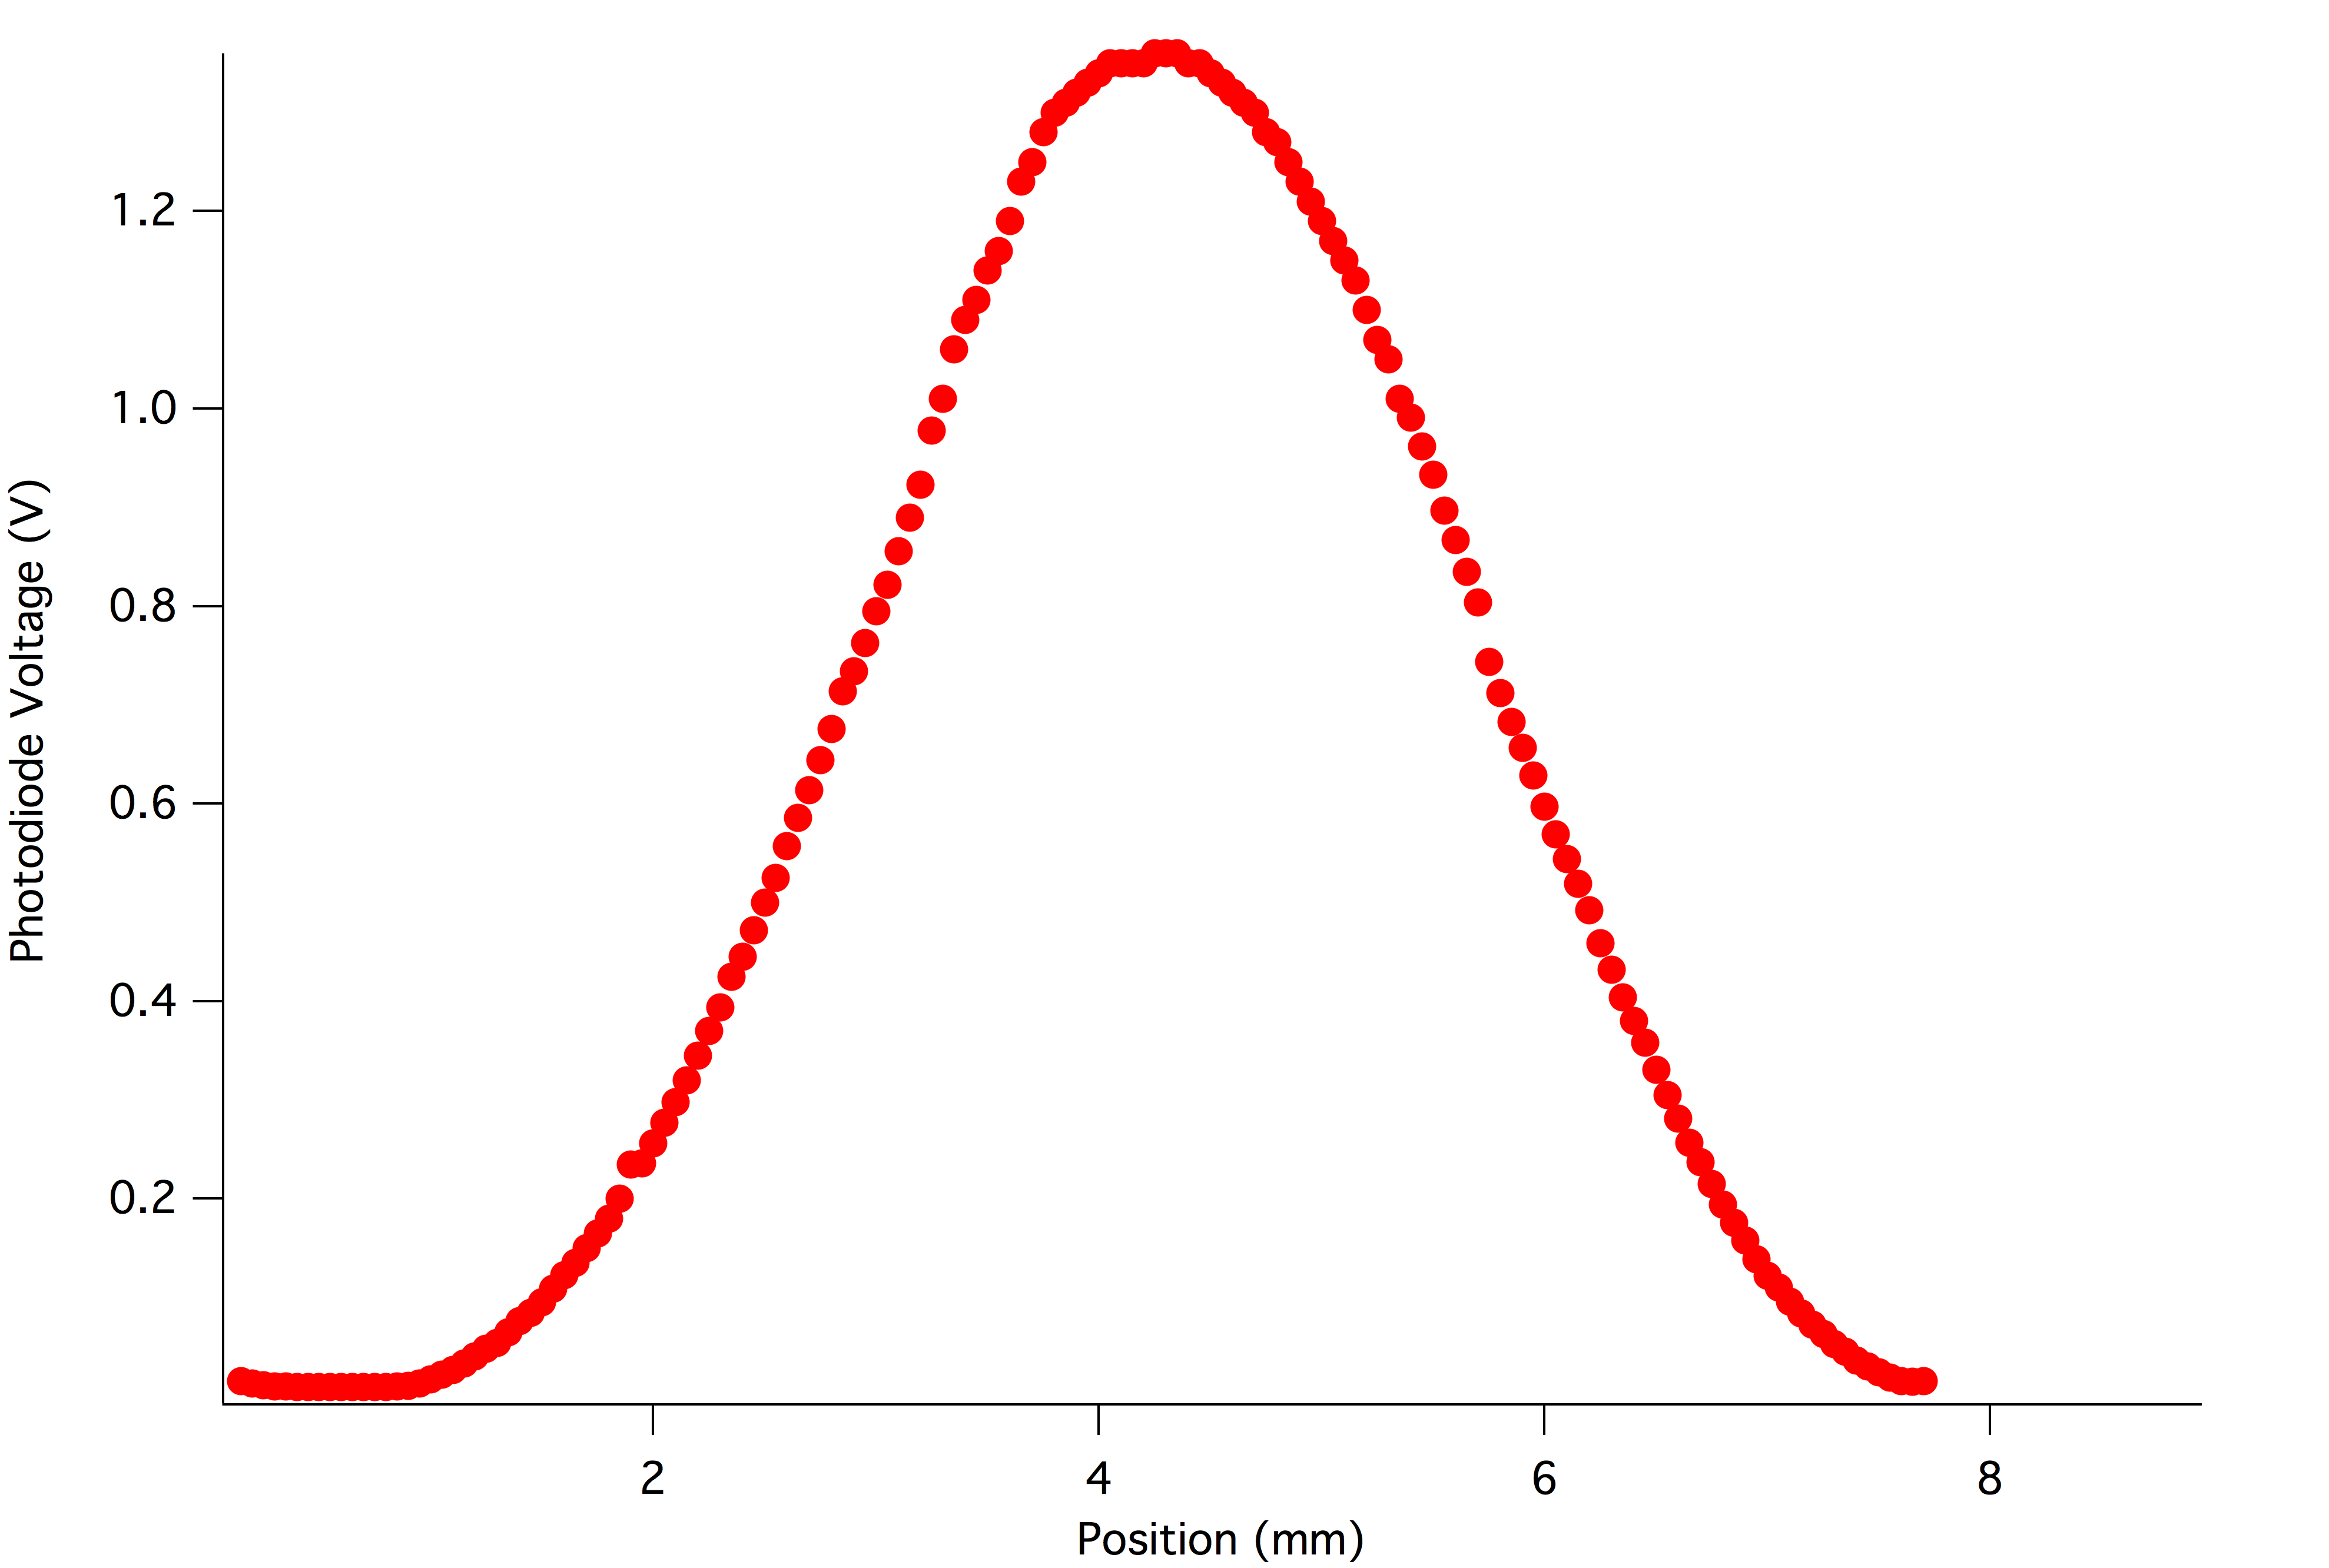
\includegraphics[width=3.2in]{singleres.png}
\caption{Recorded data for double (left) and single-slit (right) interference experiments.}
\label{ds}
\end{figure}

\newpage

The recorded raw data for the double and single-slit experiments are shown in Fig.\ref{ds}. 

Using plotting tools and a non-linear least squares curve fitting routing in Igor Pro while applying Eq. \ref{eq1}, we can obtain the plot shown below in Fig. \ref{double}. Calculation of the error bars will be included in the discussion section.

\begin{figure}[h]
\centering
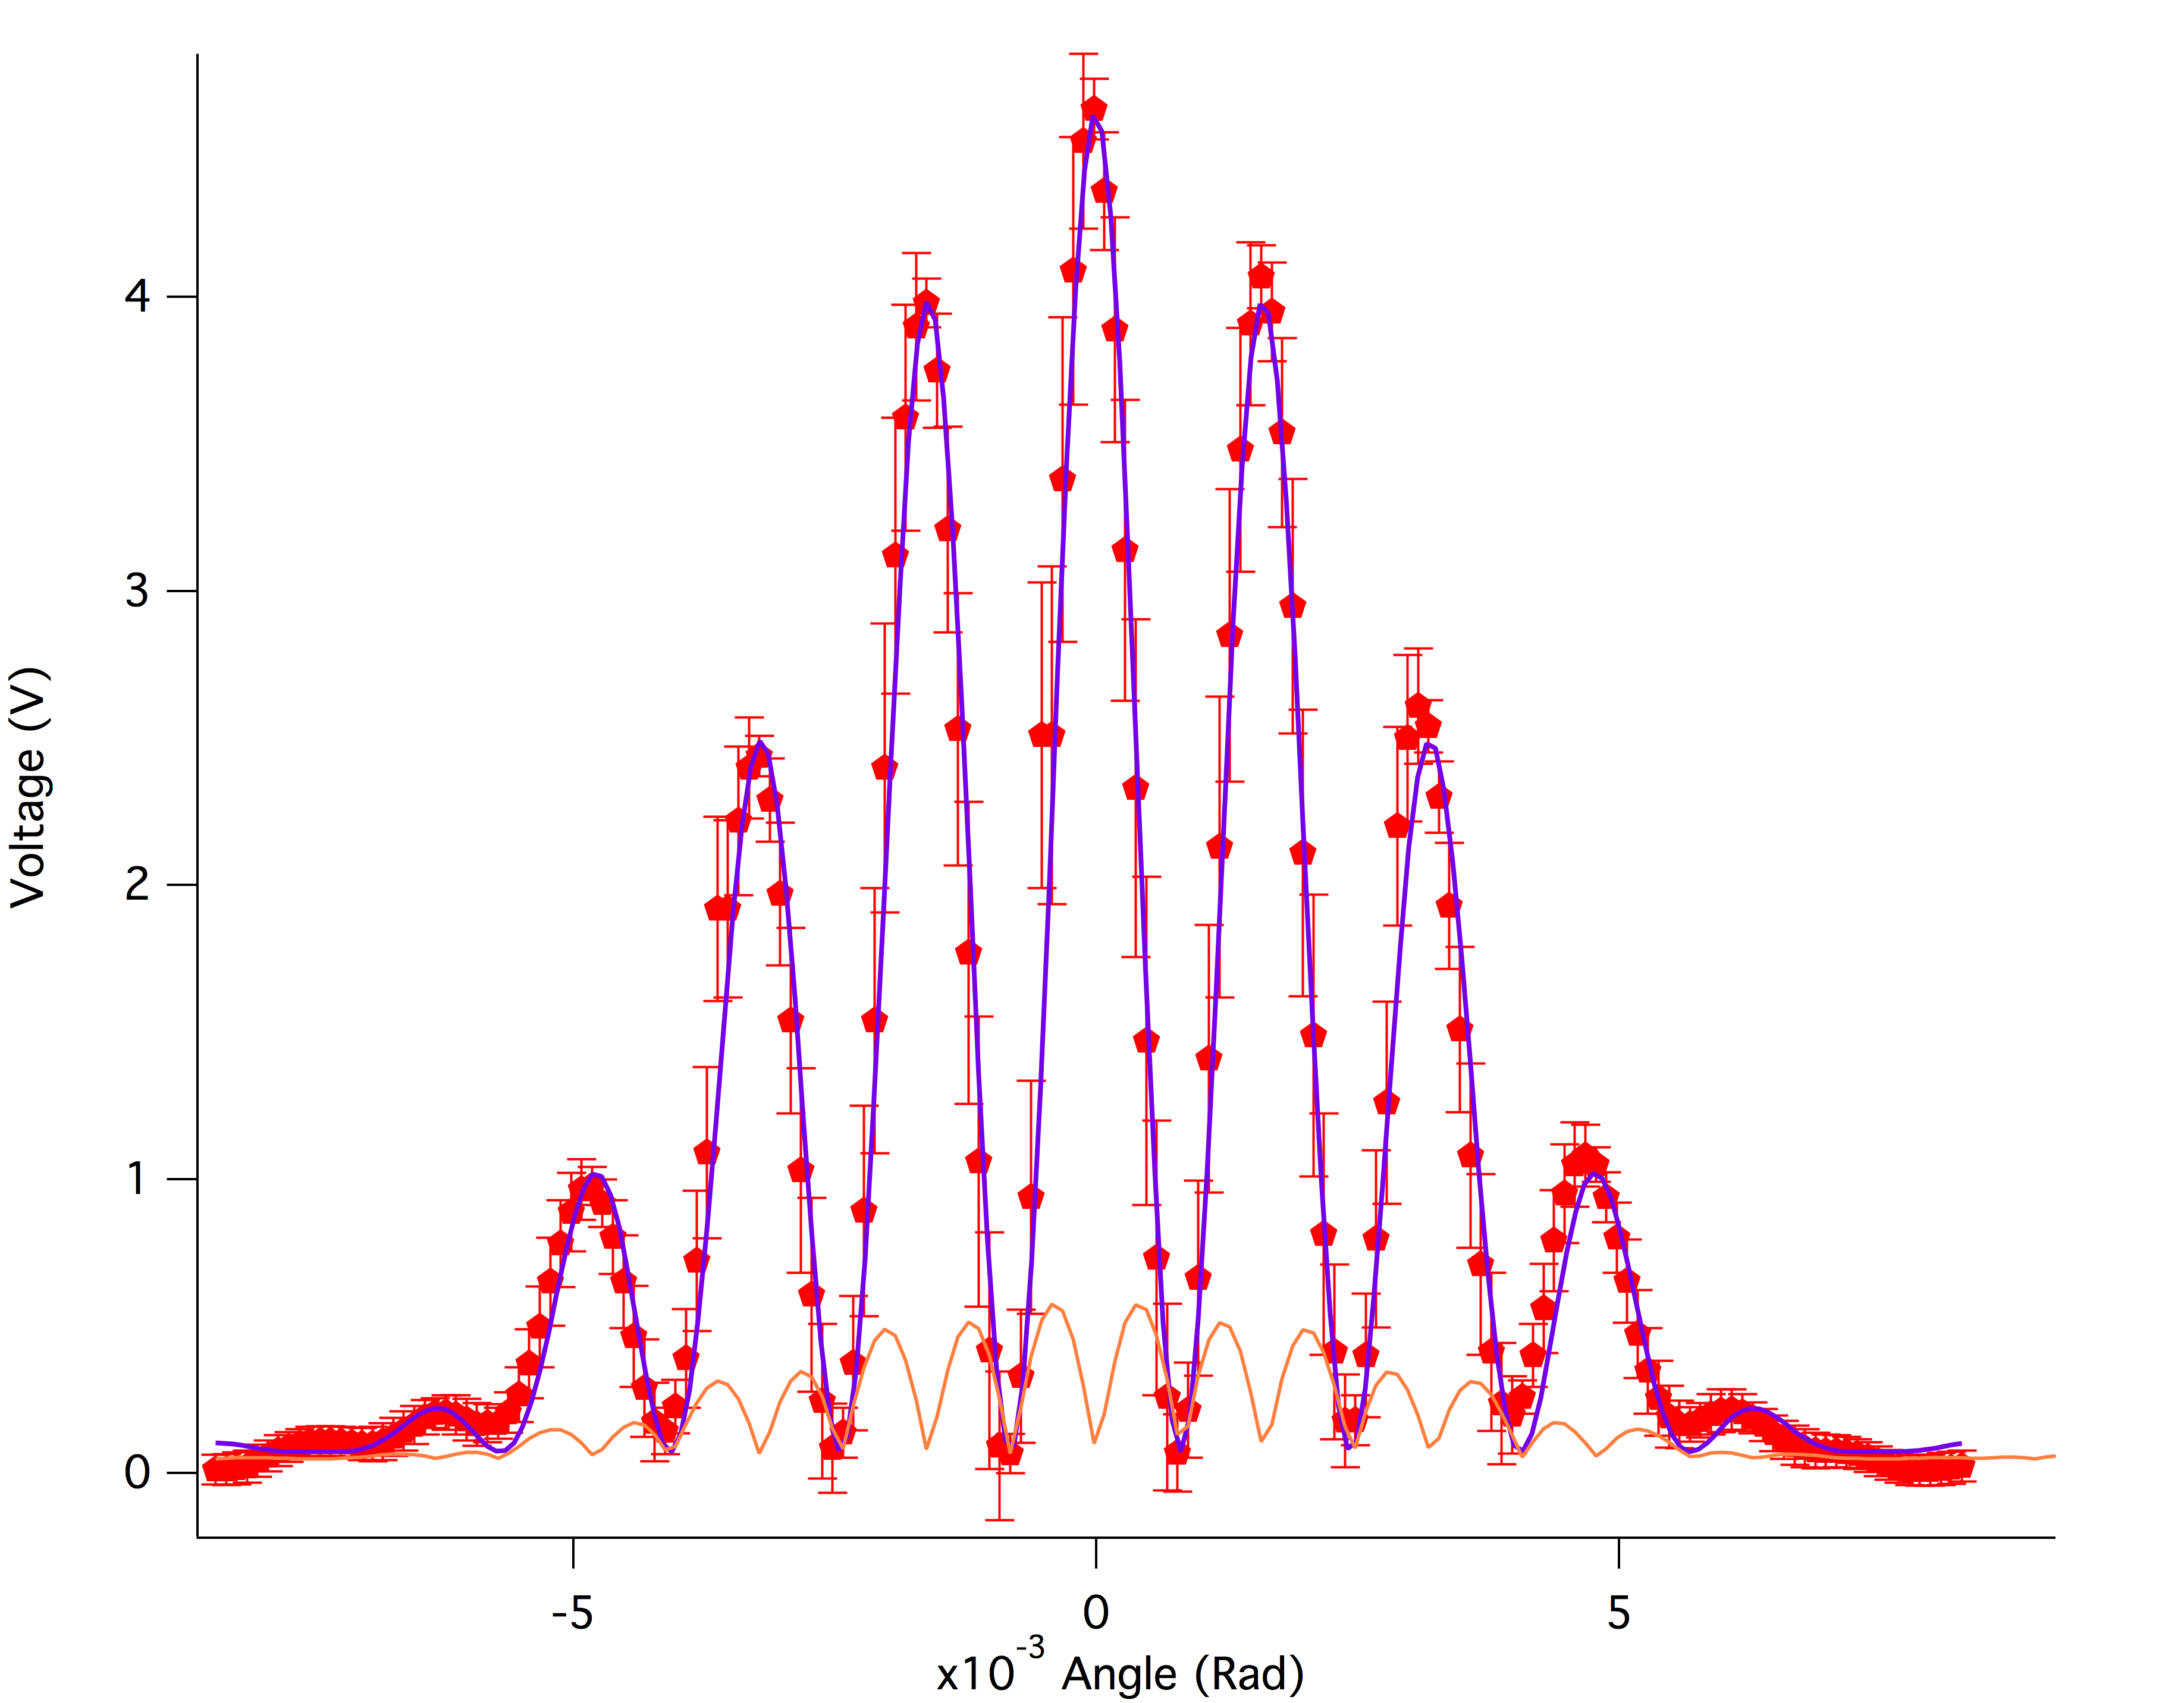
\includegraphics[width=7in]{double.png}
\caption{Plot of raw data, error bars and fit curve of the double-slit experiment. The y-axis is the voltage the photodiode outputs which is proportional to the intensity of light shining on it, and the x-axis is the angle away from the central maximum (Fig. \ref{interference}). The curve at the bottom of the graph shows the size of error as a function of angle.}
\label{double}
\end{figure}


\begin{table}[h]
\centering
\caption{Double-slit data. }
\begin{ruledtabular}
\begin{tabular}{ l c c c}
Name & Symbol & Value & Uncertainties($\pm$)\\
\hline
Slit width & a & 88.3 $\mu m$ & 0.4 $\mu m$\\
Slit separation & d & 426.89 $\mu m$ & 0.07 $\mu m$\\
Wavelength & $\lambda$ & 0.67 nm & N/A \\
Max voltage & $V_0$ & 4.55 V & 0.07 V\\
Voltage offset & $V_{offset}$ & 0.073 V & 0.008 V\\
Theta offset &$ \theta_{offset}$ & 1E-05 rad & 8E-06 rad \\
\hline
Chi Squared & $X^2$ & 0.827068&
\end{tabular}
\end{ruledtabular}
\label{data}
\end{table}

\newpage

The Fraunhofer conditions can be applied once again to create  the curve of best fit for the single-slit experiment: 

\begin{figure}[h]
\centering
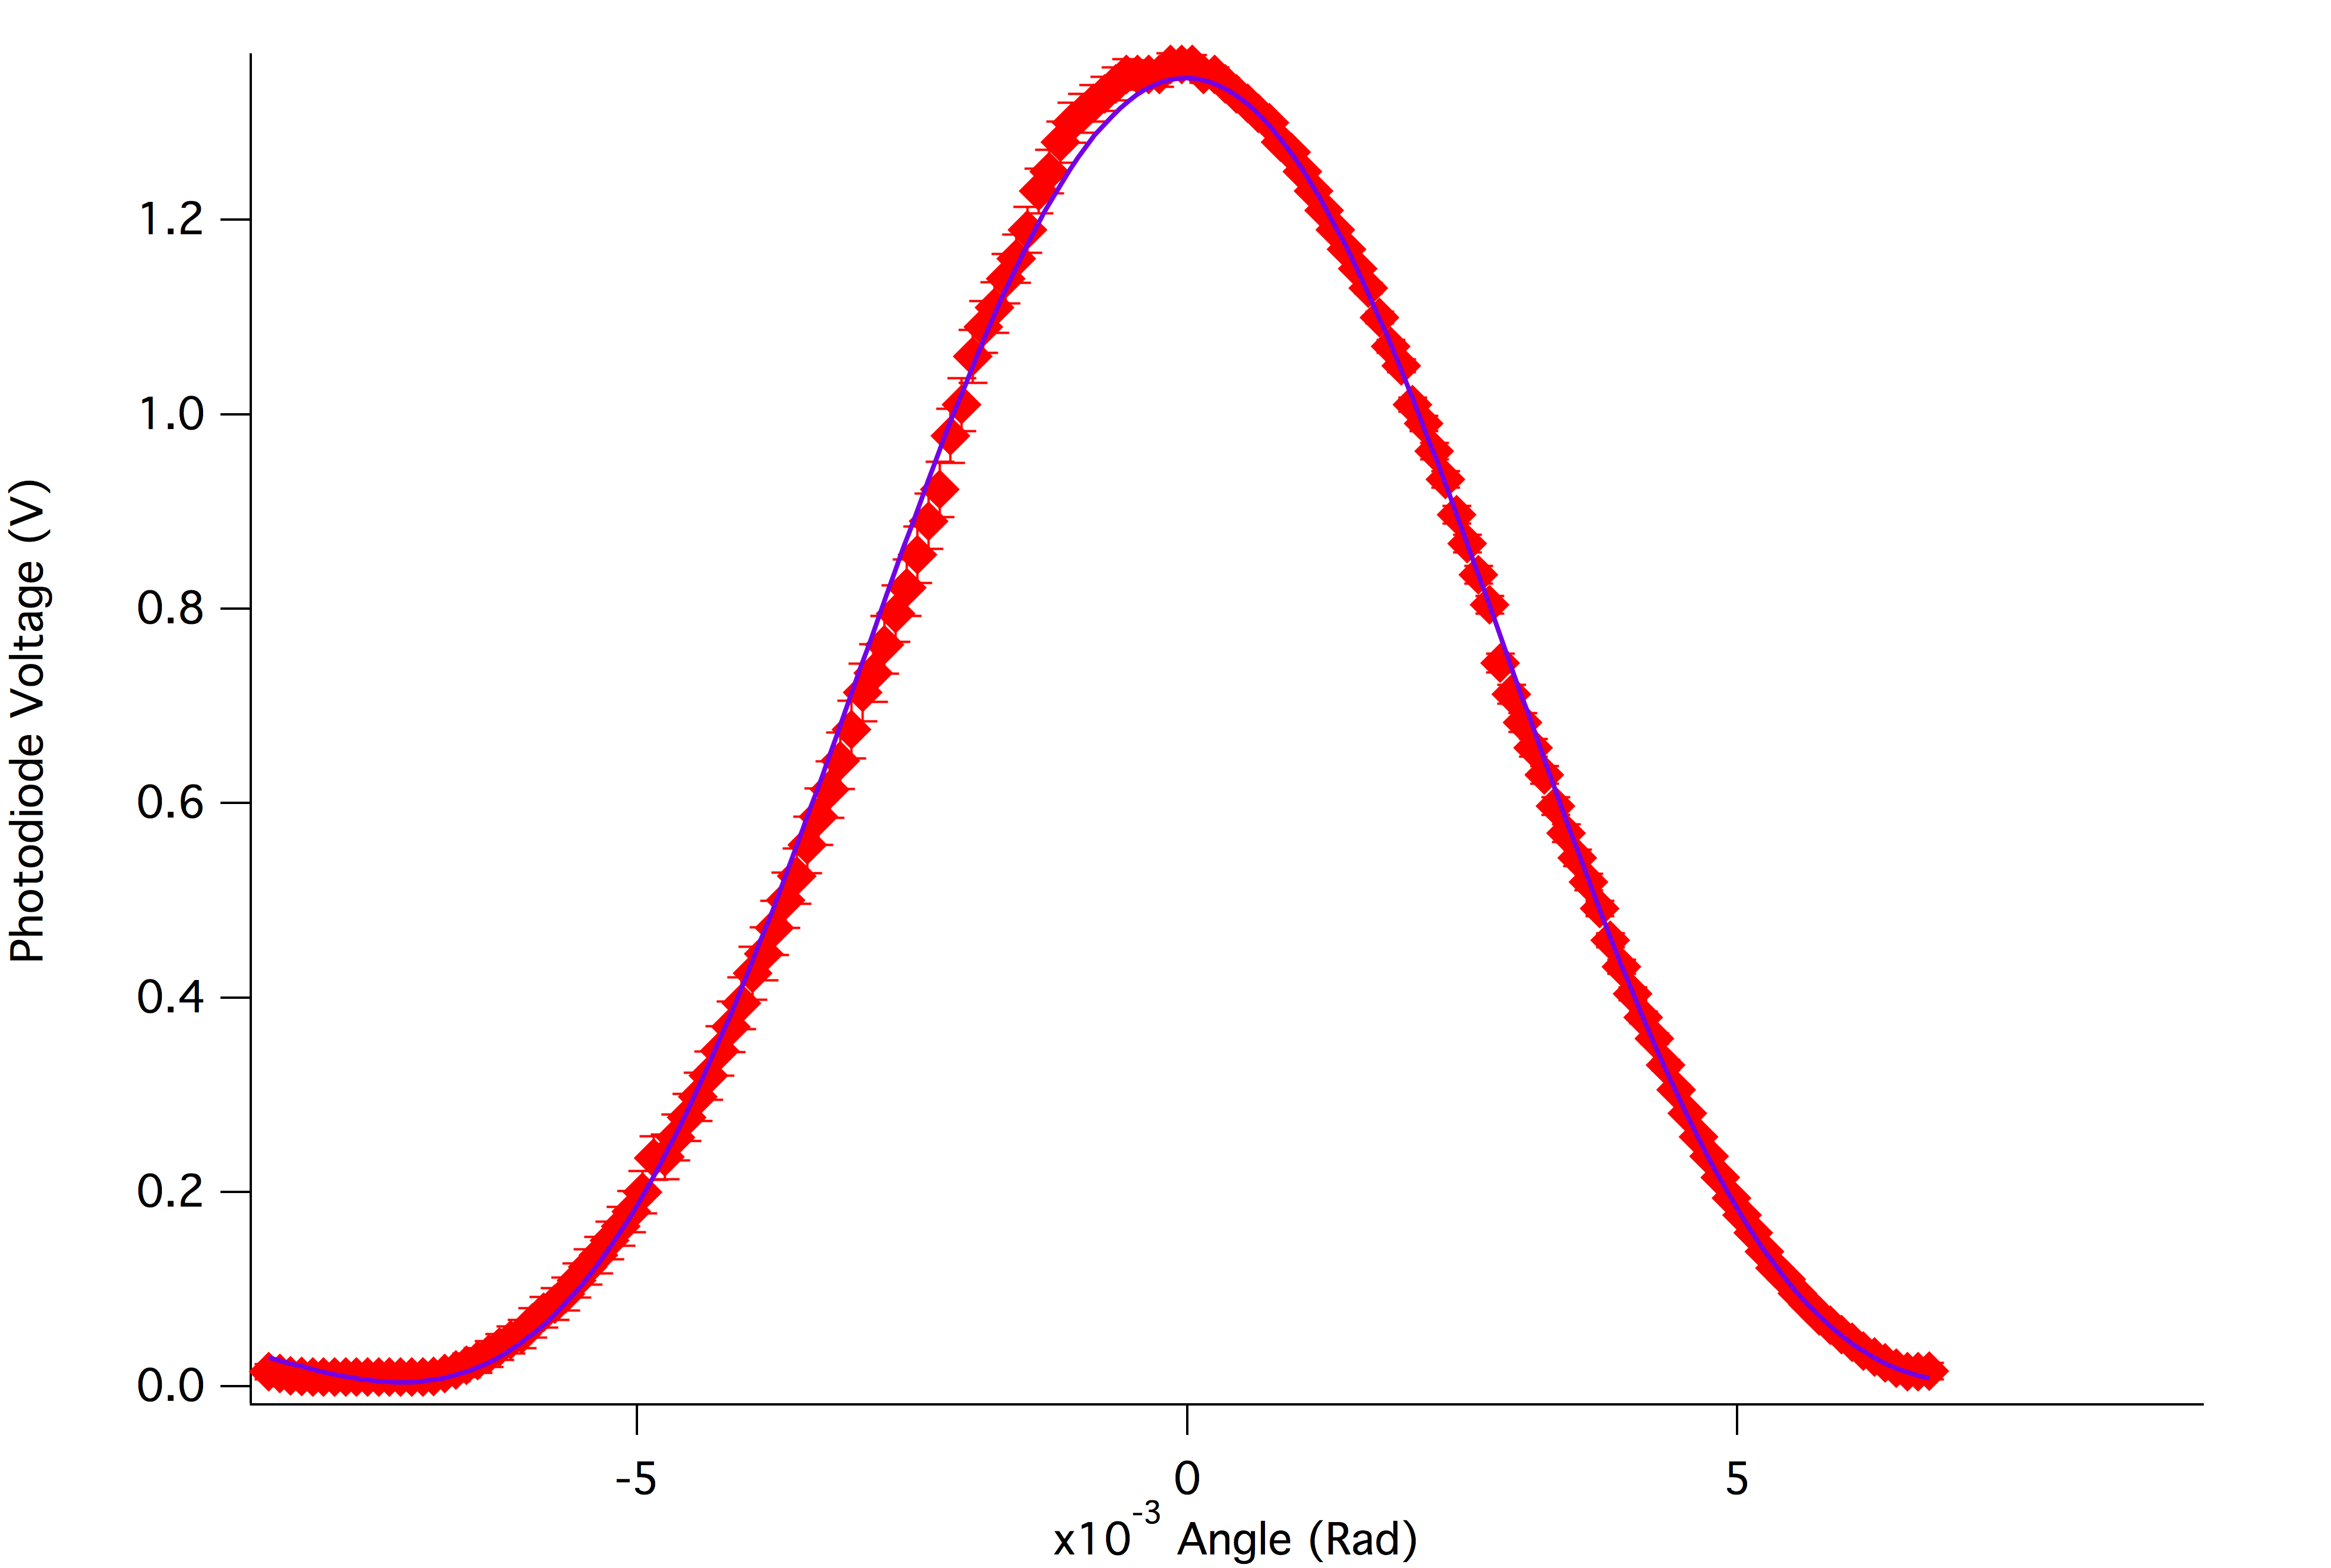
\includegraphics[width=6.6in]{single.png}
\caption{Plot of raw data, error bars and fit curve of the single-slit experiment. The y-axis is still the output voltage of the photodiode, and the x-axis is the angle away from the central maximum.}
\label{single}
\end{figure}

Using plotting tools in Igor while applying Eq.\ref{eq2}, we can obtain the plot shown in Fig.\ref{single}. Calculation of the error bars will be once again included in the discussion section for the single slit experiment.

\begin{table}[h]
\centering
\caption{Single-slit data (The definition for the two offsets will be introduced in Eq.\ref{fitdouble})}
\begin{ruledtabular}
\begin{tabular}{ l c c c}
Name & Symbol & Value & Uncertainties($\pm$)\\
\hline
Slit width & a & 93.9 $\mu m$ & 0.2 $\mu m$\\
Wavelength & $\lambda$ & 0.67 nm & N/A \\
Max voltage & $V_0$ & 1.350 V & 0.002 V\\
Voltage offset & $V_{offset}$ &  0.004 V & 0.001 V\\
Theta offset &$ \theta_{offset}$ & 1E-05 rad & 7E-06 rad \\

\hline
Chi Squared & $\chi^2$ & 1.56815 &
\end{tabular}
\end{ruledtabular}
\label{data}
\end{table}

%____________Discussion____________________________________________
\section{Discussion}

\subsection{Double-Slit Experiment}

The Fraunhofer/Fresnel theory (Eq.\ref{eq1}) of interference gives the intensity of light as a function of angle. The photodiode we use to conduct the experiment outputs a voltage proportional to the intensity of light detected ($I = kV$), thus the intensity measurements can be replaced by the voltage readings and the analysis holds for both:

\begin{equation}
V=V_0 \sinc^2( \frac{\pi a}{\lambda} \sin (\theta+\theta_{offset}))  \cos^2(\frac{\pi d}{\lambda} \sin (\theta+\theta_{offset}) + V_{offset}
\label{fitdouble}
\end{equation}

Several parameters are added to the original Fraunhofer model. $V_{offset}$ is describing the affect of the background light. Although the photodiode is kept in a closed black box, there is a slight amount of background light, which will produce an offset and shift the whole curve up. $\theta_{offset}$ describes the systematic error in angle, which is a result of the systematic error in position.\\

Some other parameters need fitting are slit width and slit separation. Due to manufacturing imperfection, the slit width and slit separation have slightly different values than given by the experiment manual. The wavelength of the laser might also be slightly off, but because equation m contains ratio terms $\frac{\pi a}{\lambda}$ and $\frac{\pi d}{\lambda}$, the numerator and denominator cannot change at the same time. Compared to a and d, $\lambda$ is less likely to have a greatly different value, so it is held at 0.67 $\mu m$. $V_{0}$ stands for the voltage measured at the central maximum.\\

Uncertainty in the variable (angle $\theta$) is determined by applying error propagation. Each step of the detector-slit change is designed to be 0.05 mm on the micrometer, from $x_i = 0.15 mm$ to $x_f = 8.35 mm$. Angle $\theta$ corresponds to the position in radian (Fig. \ref{interference}) is given by
\begin{equation}
\theta = \frac{\arctan(x-x_0)}{L}
\label{theta}
\end{equation}
$L$ is the distance from the double-slit to the photodiode, is 50 cm given by the experiment manual.
$x_0$ is found to be $4.4 \pm 0.1mm$ given by the Gaussian curve fit to the data set.

\begin{figure}[h]
\centering
\includegraphics[width=7in]{doublegaus.pdf}
\caption{Gaussian curve fit of double-slit interference is made to find the position where the intensity/output voltage of the photodiode peaks.}
\label{gasfit}
\end{figure}

We intended to advance the micrometer by $0.05 mm$ each time, but since the micrometer is controlled by human beings, each step is not perfectly $0.05 mm$, but $0.05\pm0.03 mm$.
Then the error in angle is given by taking derivative of Eq. \ref{theta} and multiply $\theta^\prime$ by $\delta x$, which is $0.03 mm$. 


\begin{equation}
\theta^\prime = \frac{1}{L(1+(x-x_0)^2)}
\label{thetaprime}
\end{equation}

\begin{equation}
\delta\theta = \theta^\prime \delta x = \frac{\delta x}{L(1+(x-x_0)^2)}
\label{deltatheta}
\end{equation}

$\delta\theta$ is a function of position x. The same method of taking derivative could be applied to find the error in voltage, but it is rather messy. So a different approach is adopted to find $\delta V$, which is to change $\theta$ in Eq. \ref{fitdouble} by $\delta\theta$ and calculate the resulting change in V, which is then divided by 2.

\begin{equation}
\delta V = \frac{\left| V(\theta+\delta\theta)-V(\theta-\delta\theta)\right |}{2}
\label{deltav}
\end{equation}

It can be seen that the same $\delta\theta$ has a smaller impact on $\delta V$ when $V^\prime$ is small, and a bigger impact when $V^\prime$ is big.\\

The multimeter itself also contributes to the error in angle. We estimate the error in meter readings to be $0.05v$.
So the overall $\delta V$ is
\begin{equation}
\delta V_{total} = \delta V+\delta V_{meter} = \delta V + 0.05v
\label{deltavtotal}
\end{equation}
$\delta V$ is plotted as a function of angle in Fig. \ref{double}.\\

The reduced $\chi^2$ is calculated for the fit curve, yielding a value of 0.827. The value is close to 1, meaning that the fit is good within estimation of error. The results confirm the Fraunhofer model for double-slit diffraction. \\

\subsection{Single-Slit Experiment}

The intensity of light as a function of $\theta$ in single-slit experiment is given by the Fraunhofer/Fresnel theory in Eq. \ref{eq2}, which can then be transformed as
\begin{equation}
V=V_0 \cos^2(\frac{\pi d}{\lambda} \sin (\theta+\theta_{offset})) + V_{offset}
\label{fitsingle}
\end{equation}
Parameters need fitting are slit width $(a)$, slit separation $(d)$, maximal voltage $(V_0)$, offset in voltage $(V_{offset})$ due to background light, and offset in $\theta$ $(\theta_{offset})$ due to systematic error of position.\\

Uncertainty is determined using the same method. $\theta$ is found using Eq. \ref{theta} while x goes from $x_i = 0.15mm$ to $x_f = 7.7mm$ with a step size of $0.05mm$. However, the value of $x_0$ need re-calculating, since the single-slit pattern is slightly shifted than the double-slit pattern. A Gaussian fit is done to the data to determine $x_{offset}$, which is $4.327 \pm 0.003mm$ (Fig. \ref{gasfit2}).\\

\begin{figure}[h]
\centering
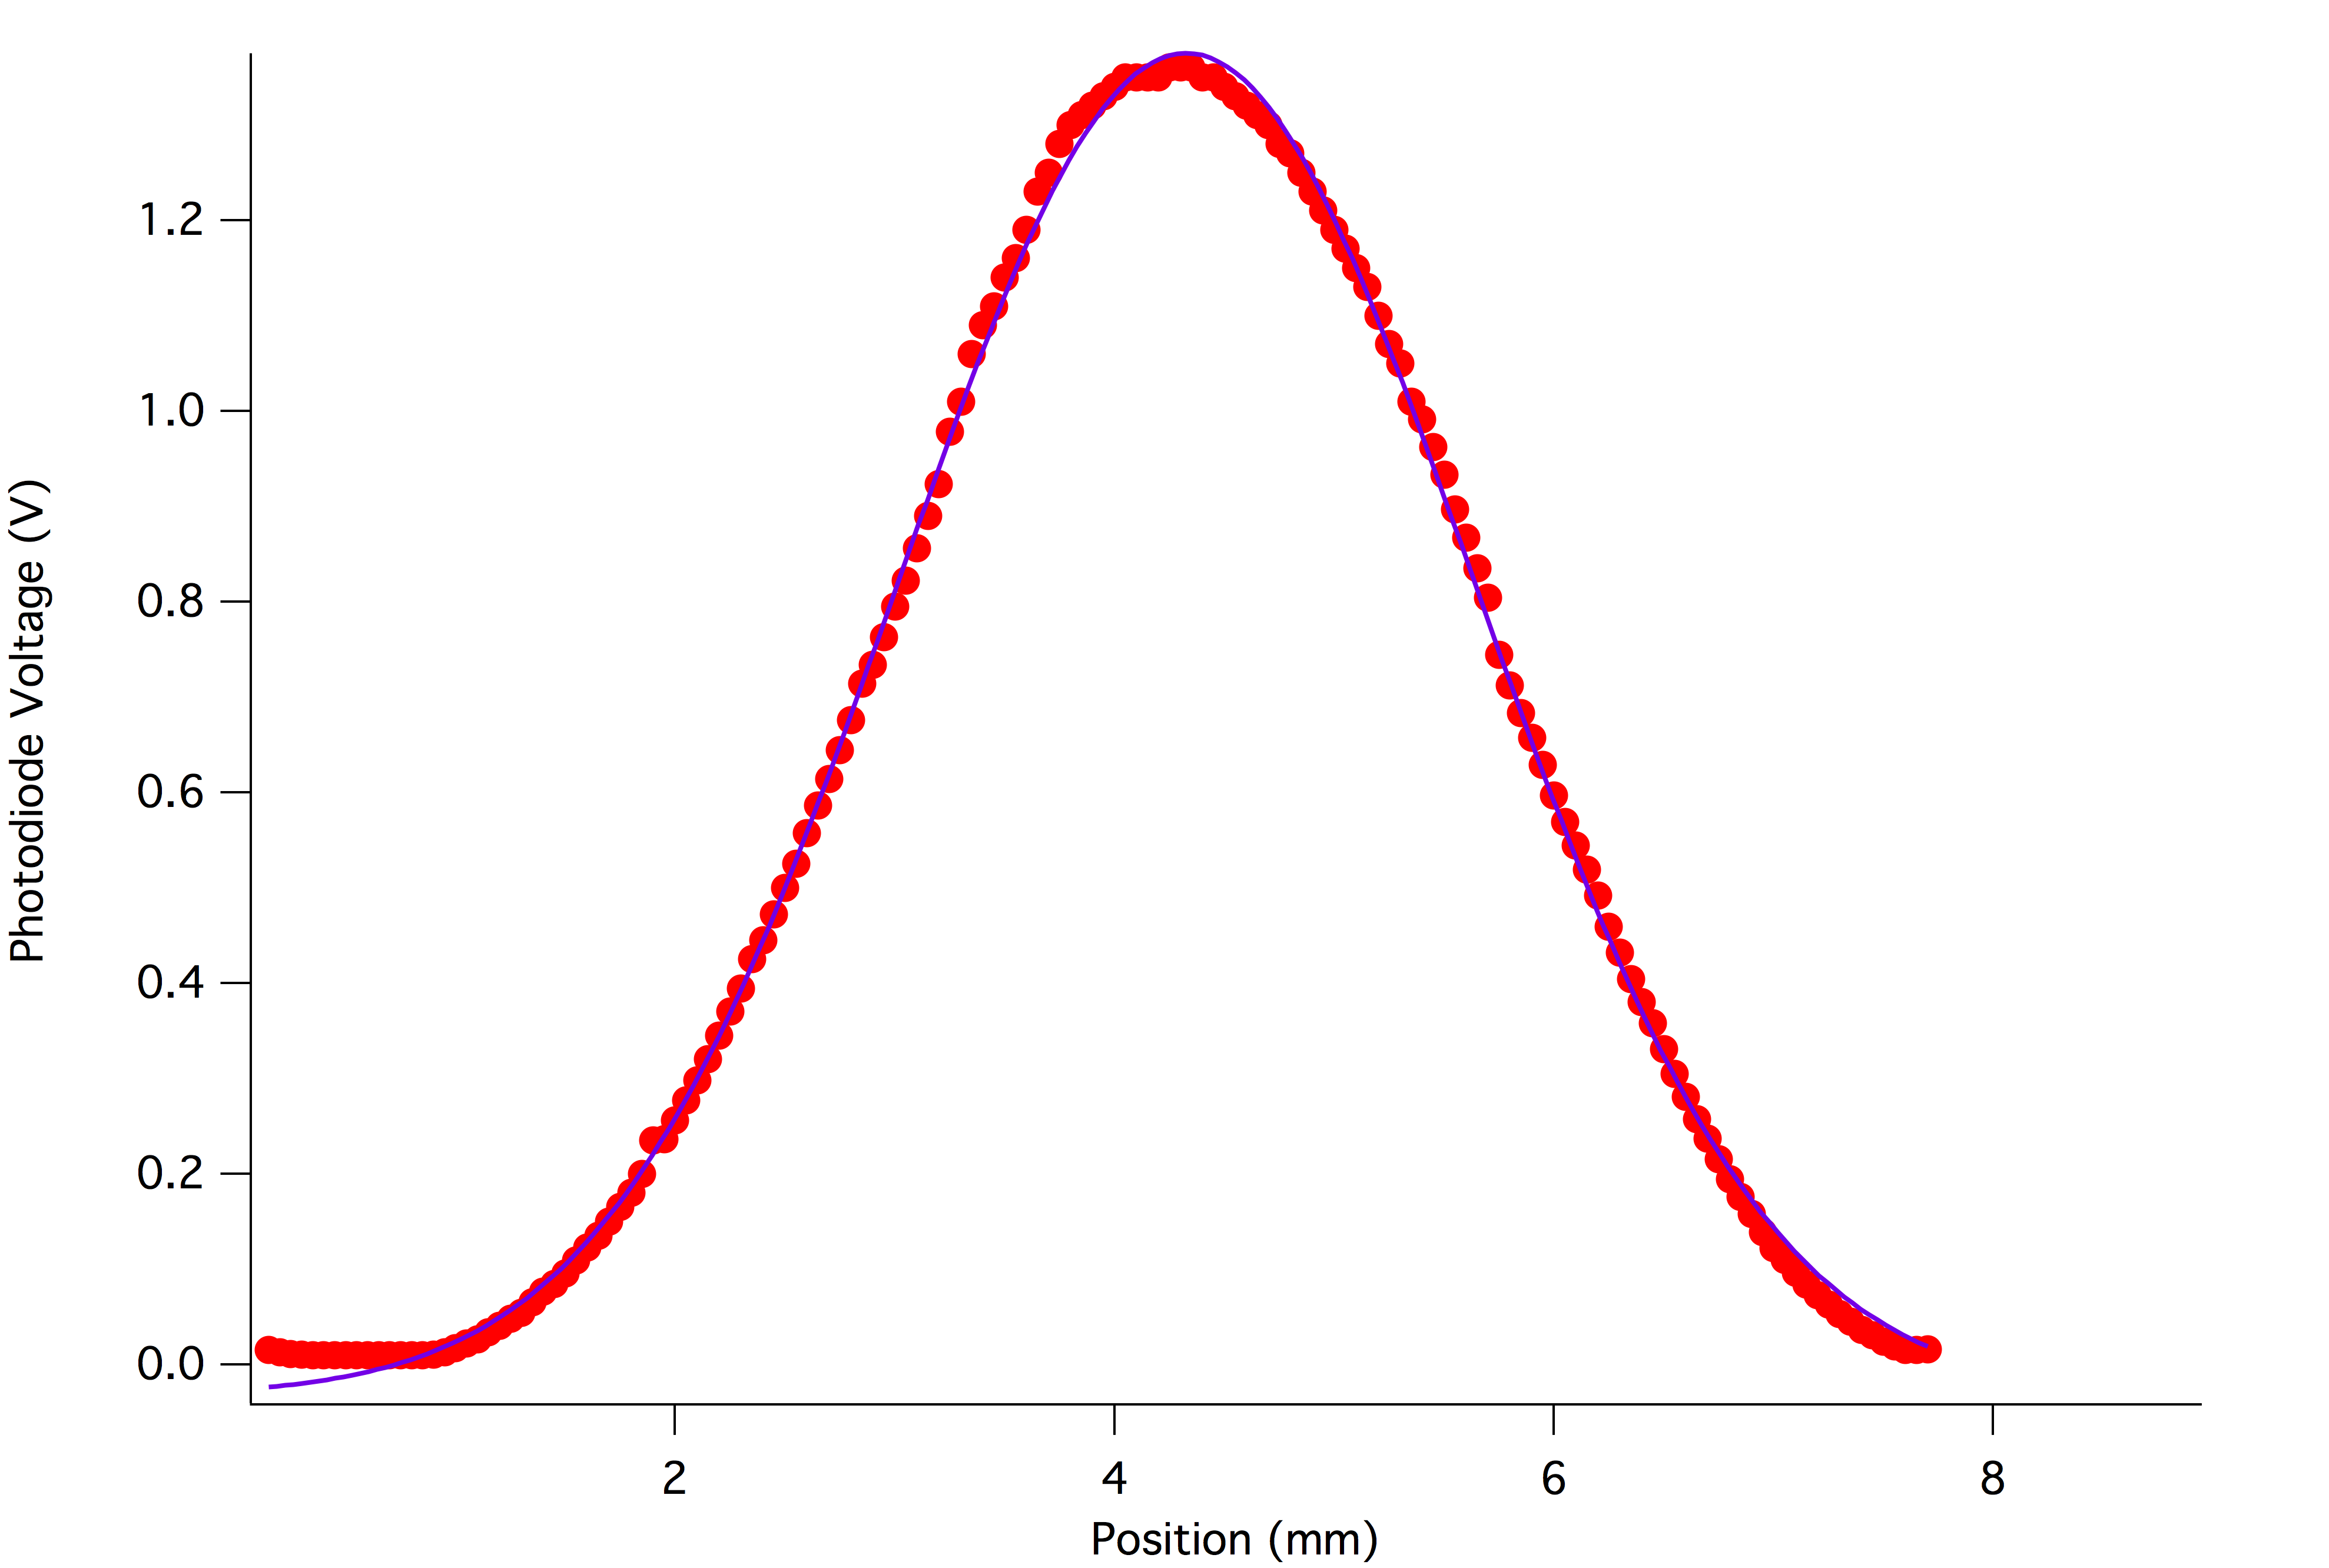
\includegraphics[width=7in]{singlegaus.png}
\caption{Gaussian curve fit of single-slit diffraction is made to find the position where intensity/output voltage of the photodiode peaks.}
\label{gasfit2}
\end{figure}

The slit to detector distance L remains $50 cm$. Uncertainty in step size is also considered to be $0.03mm$, as in the double-slit experiment. Eq. \ref{thetaprime}, \ref{deltatheta} and \ref{deltav} are used to determine uncertainty in voltage. In the final step of calculating $\delta V_{total}$ (Eq. \ref{deltavtotal}), $\delta V_{meter}$ is changed to $0.01v$, because the single-slit pattern has smaller intensity and thus a fluctuation of smaller scale in voltage.\\

The reduced $\chi^2$ is 1.56815, which indicates that if we were to redo the experiment, the possibility of getting a bigger mean values is around 0.15, given 5 degrees of freedom. This result shows that the peak position of the fit is slightly bigger than the peak position of the data. The plot confirms this, because the data points with angle smaller than 0 seem to have a systematic error, and the shape of the raw data curve is slightly skewed to the right. This error might be caused by the slit-block blocking one band of light imperfectly. But in the big picture, the data confirm the Fraunhofer model for single-slit diffraction.\\

\subsection{Comparison}

Looking at parts A and B, we see that the the maximum voltage ($V_0$) for the double-slit is approximately 4 times the maximum voltage for the single-slit equation. This is because when two central maximums of the two slits are superposed, the amplitude doubles at the central maximum ($\theta = 0$). The intensity is proportional to the amplitude squared: $$I \propto A^2 \ \ \ \	4I \propto(2A)^2$$ This relationship is clearly shown in our experiment: $$\frac{V_{0,double}}{V_{0,single}}=\frac{A_{0,double}^2}{A_{0,single}^2} = \frac{4.55\pm 0.07}{1.350 \pm 0.002}=3.37 \pm 0.06 $$ 

The signal is not quite quadrupled, may be due to photodiode saturation or tilting detector-slit, but this result does show a significantly greater central maximum intensity than if wave interference did not happen, which would give a double-slit intensity only twice as big as the single-slit one. \\




%____________Conclusion____________________________________________
\section{Conclusion}

With $\chi^2$ values of 0.827 and 1.57, the observed interference patterns of double-slit and single-slit are consistent with the Fraunhofer model, which describes far-field diffraction. This result confirms that light is wave.


\begin{acknowledgments}

We gratefully acknowledge Nathaneal Fortune and Dana Parsons, who helped with the experimentation and editing of this experiment.  This work was supported by the Smith College Physics Department.

\end{acknowledgments}


\begin{thebibliography}{99}

\bibitem{wik} Double Slit Experiment, \url{<http://upload.wikimedia.org/wikipedia/commons/c/c2/Single_slit_and_double_slit2.jpg
/>}.

\bibitem{dia} TeachSpin Instructions Manual,\textit{Two-Slit interference, One Photon at a Time (TWS1-B), Pulse Counter/Interval Timer (PCIT1)}, 6/2013.
\bibitem{interference} Young Two-Slit Experiment, \url{http://abyss.uoregon.edu/~js/21st_century_science/lectures/lec13.html}

\end{thebibliography}

%\newpage   % Start a new page for tables

\end{document}
